\section{Rings}

  \begin{definition}[Ring]
    A \textbf{ring} is a set $(R, +, \times)$ equipped with two operations, called addition and multiplication. It has properties: 
    \begin{enumerate}
      \item $R$ is an abelian group with respect to $+$, where we denote the additive identity as $0$ and the additive inverse of $x$ as $-x$. 
      \item $R$ is a monoid with respect to $\times$, where we denote the multiplicative identity as $1$, also known as the \textbf{unity}. 
      \item $\times$ is both left and right distributive with respect to addition $+$
      \begin{align}
        a \times (b + c) & = a\times b + a\times c \\ 
        (a + b) \times c & = a\times c + b\times c 
      \end{align}
      for all $a, b, c \in \mathbb{R}$. 
    \end{enumerate} 
    If $\times$ is associative, $R$ is called an \textbf{associative ring}, and if $\times$ is commutative, $R$ is called a \textbf{commutative ring}. 
  \end{definition}

  In fact, in some cases the existence of the multiplicative identity is not even assumed, though we will do it here.\footnote{If a multiplicative identity is not assumed, then this is called an \textit{rng}, or a \textit{rung}.}

  \begin{lemma} 
    Additive inverses are unique and $-1 \times a$ is the additive inverse of $a$. 
  \end{lemma}
  \begin{proof}
    We can see that 
    \begin{align}
      -1 + 1 = 0 & \implies (-1 + 1) \times a = 0 \times a \\
                 & \implies -1 \times a + 1 \times a = 0 \\
                 & \implies -1 \times a + a = 0 
    \end{align}
    and therefore by definition $-1 \times a$ must be the additive inverse. 
  \end{proof} 

  Note that we do not assume that there exists multiplicative inverses in a ring. However, there may be some elements for which multiplicative inverses do exist, i.e. $a, b \in R$ where $ab = 1$.  

  \begin{definition}[Unit]
    A \textbf{unit} of a ring $R$ is an element $u \in R$ that has a multiplicative inverse in $R$. That is, there exists a $v \in R$ s.t. $uv = vu = 1$. 
  \end{definition}

  The next property that we would like to talk about is a zero divisor, which is the property that nonzero $a, b \in R$ satisfy $ab = 0$. 

  \begin{definition}[Left, Right Zero Divisor]
    An element $a$ of a ring $R$ is called a \textbf{left zero divisor} if there exists a nonzero $x$ such that $a x = 0$ and a \textbf{right zero divisor} if there exists a nonzero $x$ such that $x a = 0$. 
  \end{definition} 

  Another property that we would desire is some sort of decomposition of ring elements as other ring elements. 

  \begin{definition}[Left, Right Divisor]
    Let $a, b \in R$ a ring. 
    \begin{enumerate}
      \item If there exists an element $x \in R$ with $ax = b$, we say $a$ is a \textbf{left divisor} of $b$. 

      \item If there exists an element $y \in R$ with $ya = b$, we say $a$ is a \textbf{right divisor} of $b$. 

      \item We say $a$ is a \textbf{two-sided divisor} if it is both a left divisor and a right divisor of $b$. Note that the $x$ and $y$ are not required to be equal. 
    \end{enumerate}
  \end{definition}

  It turns out that the existence of units and zero divisors classify rings into subcategories, which we will elaborate on. That is, we will start with the most general theory on rings, and then shrink down into subcategories of rings. 

  \begin{figure}[H]
    \centering 
    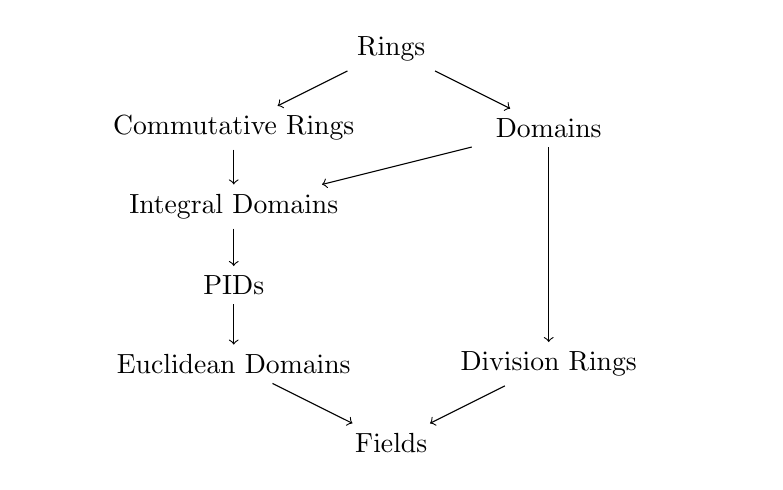
\begin{tikzpicture}[
        node distance=2cm,
        box/.style={
            text width=5cm,
            align=center
        }
    ]
        % Nodes for ring types
        \node[box] (rings) at (0,0) {Rings};
        \node[box] (comm) at (-2,-1) {Commutative Rings};
        \node[box] (domains) at (2,-1) {Domains};
        \node[box] (int) at (-2,-2) {Integral Domains};
        \node[box] (divring) at (2,-4) {Division Rings};
        \node[box] (pid) at (-2,-3) {PIDs};
        \node[box] (euc) at (-2,-4) {Euclidean Domains};
        \node[box] (fields) at (0,-5) {Fields};
        
        % Left path arrows
        \draw[->] (rings) -- (comm);
        \draw[->] (comm) -- (int);
        \draw[->] (int) -- (pid);
        \draw[->] (pid) -- (euc);
        \draw[->] (euc) -- (fields);
        \draw[->] (divring) -- (fields);
        
        % Right path arrows
        \draw[->] (rings) -- (domains);
        \draw[->] (domains) -- (int);
        \draw[->] (domains) -- (divring);
    \end{tikzpicture}
    \caption{Basic hierarchy of rings.} 
    \label{fig:ring_hierarchy}
  \end{figure} 

\subsection{Well-Known Rings}

  We list some classic examples of rings.

  \begin{definition}[Integers]
    The ring of integers $\mathbb{Z}$ consists of:
    \begin{enumerate}
      \item The set $\{\dots,-2,-1,0,1,2,\dots\}$
      \item Binary operations:
      \begin{equation}
        + : \mathbb{Z} \times \mathbb{Z} \to \mathbb{Z} \text{ (addition)}
      \end{equation}
      \begin{equation}
        \cdot : \mathbb{Z} \times \mathbb{Z} \to \mathbb{Z} \text{ (multiplication)}
      \end{equation}
      \item Additive identity 0
      \item Multiplicative identity 1
    \end{enumerate}
    This forms a commutative ring with unity that is also an integral domain.
  \end{definition}

  \begin{definition}[Gaussian Integers]
    The ring of Gaussian integers $\mathbb{Z}[i]$ consists of:
    \begin{enumerate}
      \item The set $\{a + bi : a,b \in \mathbb{Z}\}$ where $i^2 = -1$
      \item Complex addition and multiplication
      \item Additive identity $0 + 0i$
      \item Multiplicative identity $1 + 0i$
    \end{enumerate}
    This forms a commutative ring with unity that is also a unique factorization domain.
  \end{definition}

  \begin{definition}[Rationals, Reals, Complexes]
    The fields $\mathbb{Q}$, $\mathbb{R}$, and $\mathbb{C}$ are rings with:
    \begin{enumerate}
      \item Sets: 
        \begin{itemize}
          \item $\mathbb{Q}$: rational numbers $\{\frac{a}{b} : a,b \in \mathbb{Z}, b \neq 0\}$
          \item $\mathbb{R}$: real numbers
          \item $\mathbb{C}$: complex numbers $\{a + bi : a,b \in \mathbb{R}\}$
        \end{itemize}
      \item Standard addition and multiplication
      \item Additive identity 0
      \item Multiplicative identity 1
    \end{enumerate}
    These form commutative rings with unity where every non-zero element has a multiplicative inverse.
  \end{definition}

  \begin{definition}[Continuous Functions]
    The set of all continuous functions $f: \mathbb{R} \rightarrow \mathbb{R}$ is a ring under point-wise addition and multiplication. 
  \end{definition}

  The product of two finitary sequences $(a_0, a_1, a_2, ...)$ and $(b_0, b_1, b_2, ...)$ in the ring $F[x]$ is a sequence 
  \begin{equation}
    (c_0, c_1, c_2, ...), \; c_k = \sum_{l = 0}^{k} a_l b_{k-l}
  \end{equation}
  This formula works for infinite (non-finitary) sequences too. 

  \begin{definition}[Power Series]
    For a ring $R$, the \textbf{ring of formal\footnote{This is called ``formal'' since we just think of its as any series and do not require convergence like we do in analysis.} power series over $R$}, denoted $R[[x]]$, consists of 
    \begin{enumerate}
      \item Elements called \textbf{power series} which are formal expressions of the form 
      \begin{equation}
        a_0 + a_1 x + a_2 x^2 + a_3 x^3...
      \end{equation}

      \item Addition is defined component-wise. 

      \item Multiplication is defined the same for univariate polynomials. 
    \end{enumerate}
  \end{definition}

  \begin{definition}[P-Adic Integers]
    For a prime p, the ring of p-adic integers $\mathbb{Z}_p$ consists of:
    \begin{enumerate}
      \item The set of formal power series $\sum_{i=0}^{\infty} a_i p^i$ where $a_i \in \{0,1,\dots,p-1\}$
      \item Binary operations extending natural addition and multiplication modulo powers of p
      \item Additive identity 0
      \item Multiplicative identity 1
    \end{enumerate}
    This forms a complete, commutative ring with unity.
  \end{definition}

  \begin{definition}[Matrices]
    The ring $M_n(R)$ of $n \times n$ matrices over a ring $R$ consists of:
    \begin{enumerate}
      \item $n \times n$ arrays of elements from $R$
      \item Matrix addition (entry-wise):
      \begin{equation}
        (A + B)_{ij} = A_{ij} + B_{ij}
      \end{equation}
      \item Matrix multiplication:
      \begin{equation}
        (AB)_{ij} = \sum_{k=1}^n A_{ik}B_{kj}
      \end{equation}
      \item Zero matrix as additive identity
      \item Identity matrix $I_n$ as multiplicative identity
    \end{enumerate}
    This forms a non-commutative ring for $n > 1$, even when $R$ is commutative.
  \end{definition}

  \begin{theorem}[Power Set]
    Given a set $X$, let $2^X$ be its power set, that is the set of all subsets of $X$. Then, $2^X$ is a commutative associative ring with respect to the operations of symmetric difference (i.e. the set of elements which is in exactly one of the sets) 
    \begin{equation}
      M \bigtriangleup N \equiv (M \setminus N) \cup (N \setminus M)
    \end{equation}
    and intersection $\cap$, taken for addition an multiplication, respectively. 
  \end{theorem}
  \begin{proof}
    We will not prove all of the axioms of the ring, but we can state some important facts about this structure. The additive identity is $\emptyset$ and the multiplicative identity is $X$. Finally, it is clear that 
    \begin{align*}
      & M \bigtriangleup N \equiv (M \setminus N) \cup (N \setminus M) \equiv N \bigtriangleup M \\
      & M \cap N = N \cap M \\
      & M \cap N \cap P = (M \cap N) \cap P = M \cap (N \cap P)
    \end{align*}
  \end{proof}  

\subsection{Commutative Rings} 

  Note that for commutative rings, distinguishing left and right divisors are meaningless, and so we can talk about just \textit{divisors}. 

  \begin{lemma}[Left=Right Divisors]
    In a commutative ring $R$, $a$ is a left divisor of $b$ iff $a$ is a right divisor of $b$. In this case, we just say that $a$ is a \textbf{divisor} of $b$, written $a | b$. 
  \end{lemma}
  \begin{proof}
    $a$ is a right divisor of $b \iff \exists x (xa = b) \iff \exists x (ax = b) \iff a$ is a left divisor. 
  \end{proof} 

  \begin{definition}[Greatest Common Divisor]
    The \textbf{greatest common divisor} of elements $a$ and $b$ of an integral domain is a common divisor of $a$ and $b$ divisible by all their common divisors. It is denoted GCD$(a, b)$. If $\mathrm{gcd}(a, b) = 1$, then $a$ and $b$ are said to be \textbf{relatively prime}. 
  \end{definition} 

  \begin{definition}[Prime and Compositive Elements]
    In a commutative ring $R$, an element $p \in R$ is said to be \textbf{prime} if it is not $0$, not a unit, and has only divisors $1$ and $p$. 
  \end{definition}

  \begin{lemma}[Euclid]
    If $p$ is prime, then $p|ab \implies p|a$ or $p|b$.  
  \end{lemma}

  \begin{lemma} 
    Let $R$ be a commutative ring and $a, b, d \in R$. If $d|a$ and $d|b$, then $d | (ma + nb)$ for any $m, n \in R$. 
  \end{lemma} 

  \begin{theorem}[Commutativity Transfers to Polynomials]
    If $R$ is a commutative ring, then $R[x]$ is a commutative ring. 
  \end{theorem}

  \begin{theorem}[Single Factor Theorem]
    Given a commutative ring $R$ with $p \in R[x]$, if $p(r) = 0$, then $p$ can be factored in the form 
    \begin{equation}
      p(x) = (x - r) q(x)
    \end{equation}
    for some $q \in R[x]$ of degree $\mathrm{deg}(p) - 1$.\footnote{Note that this is not true for an arbitrary ring. $R$ must be commutative at least. }
  \end{theorem}

\subsection{Domains}

  We can see that domains behave similarly to the integers, but with the missing property that $\times$ is commutative. This motivates the following definition of an integral domain, which can be seen as a generalization of the integers. 

  \begin{definition}[Domain]
    A ring $R$ with no zero divisors for every element is called a \textbf{domain}. 
  \end{definition} 

  \begin{theorem}[Bounds on Degrees From Operations]
    Given that $R$ is a domain and $f, g \in R[x]$, 
    \begin{align}
      \text{deg}(f+g) & \leq \text{max}\{\text{deg}\,f, \text{deg} \,g\} \\
      \text{deg} \,f g & = \text{deg} \,f + \text{deg} \,g
    \end{align}
  \end{theorem}
  \begin{proof}
    The first is true for all rings $R$. The second may not be true if $R$ has zero divisors. 
  \end{proof}


\subsection{Integral Domains}

  \begin{definition}[Integral Domain]
    An \textbf{integral domain} is a commutative domain $R$. 
  \end{definition} 

  \begin{example}[Domains vs Integral Domains]
    We show some examples of integral domains. 
    \begin{enumerate}
      \item The ring $\mathbb{Z}$ of integers. 
      \item The field $\mathbb{R}$. 
      \item The ring $\mathbb{Z}[x]$ of polynomials of one variable with integer coefficients. 
    \end{enumerate}
    We show examples of domains that are not integral domains. 
    \begin{enumerate}
      \item Quaternions $\mathbb{H}$ are not commutative but are a domain. 
    \end{enumerate}
  \end{example} 

  \begin{theorem}[Fields are Integral Domains]
    Every field is an integral domain. 
  \end{theorem}
  \begin{proof}
    
  \end{proof}

  \begin{theorem}[Polynomial Integral Domains]
    Rings of polynomials are an integral domain if the coefficients come from an integral domain. 
  \end{theorem}
  \begin{proof}
    
  \end{proof} 

  Factorization of polynomials over $\mathbb{C}$ into linear factors and polynomials over $\mathbb{R}$ into linear and quadratic factors is similar to the factoring of the integers to prime numbers. In fact, such a factorization exists for polynomials over any field $F$, but their factors can be of any degree. Moreover, there exists no general solution for the factoring of polynomials over any field. 

  \begin{example}
    $\mathbb{Z}$ and $F[x]$ over field $F$ are integral domains. Any field $F$ is also an integral domain. 
  \end{example}

  \begin{example}
    The quotient ring $\mathbb{Z}_n$ is not an integral domain when $n$ is composite. 
  \end{example}

  \begin{example}
    A product of two nonzero commutative rings with unity $R \times S$ is not an integral domain since $(1,0) \cdot (0, 1) = (0, 0) \in R \times S$. 
  \end{example}

  \begin{example}
    The ring of $n \times n$ matrices over any nonzero ring when $ n \geq 2$ is not an integral domain. Given matrices $A, B$, if the image of $B$ is in the kernel of $A$, then $A B = 0$.
  \end{example}

  \begin{example}
    The ring of continuous functions on the interval is not an integral domain. To see why, notice that given the piecewise functions 
    \begin{equation}
      f (x) = \begin{cases}
      1 - 2x & x \in [0, \frac{1}{2}] \\
      0 & x \in [\frac{1}{2}, 1] 
      \end{cases}, \; \;\;g (x) = \begin{cases}
      0 & x \in [0, \frac{1}{2}] \\
      2x - 1 & x \in [\frac{1}{2}, 1] 
      \end{cases}
    \end{equation}
    $f, g \neq 0$, but $f g = g f = 0$. 
  \end{example}

  \begin{proposition}
    An integral domain is a ring that is isomorphic to a subring of a field. 
  \end{proposition}

  \begin{proposition}
    The characteristic of an integral domain is either $0$ or a prime number. 
  \end{proposition}

  \begin{definition}
     An element $r$ of a ring $R$ is \textbf{regular} if the mapping 
     \begin{equation}
       \rho: R \longrightarrow R, \; x \mapsto x r
     \end{equation}
    is injective for all $x \in R$. 
  \end{definition}

  \begin{proposition}
    An integral domain is a commutative associative ring where every element is regular. 
  \end{proposition}

  \begin{definition}
    Let $A$ be an integral domain. An element $a \in A$ is \textbf{divisible} by $b \in A$, denoted $b | a$ if there exists an element $q \in A$ such that $a = q b$. Elements $a$ and $b$ are \textbf{associated}, denoted $a \sim b$ if either of the following equivalent conditions holds
    \begin{enumerate}
        \item $a | b \text{ and } b | a$
        \item $a = c b, \text{ where } c$ is invertible
    \end{enumerate}
    The two conditions are equivalent because $c$ and $c^{-1}$ are both in $A$. 
  \end{definition}

\subsection{Ideals and Quotient Rings}

  \begin{definition}[Ideals]
    For an arbitrary ring $(R,+, \cdot)$, let $(R, +)$ be its additive group. A subset $I$ is a 
    \begin{enumerate}
      \item \textbf{left ideal} of $R$ if $(I, +)$ is a subgroup of $(R, +)$, and For every $r \in R$ and every $x \in I$ the left product $r \cdot x \in I$. 
      \item \textbf{right ideal} of $R$ if $(I, +)$ is a subgroup of $(R, +)$, and for every $r \in R$ and every $x \in I$, the right product $r \cdot x \in I$. 
      \item \textbf{two-sided ideal}, or an \textbf{ideal}, of $R$ if it is both a left and a right ideal. 
    \end{enumerate}
  \end{definition}

  Note that left and right modules are equivalence relations defined on a ring.\footnote{A left/right ideal can also be seen as a left/right $R$-submodule of $R$ viewed as an $R$-module. } 

  \begin{proposition}
    Every right or left ideal of a commutative ring is a two sided ideal. 
  \end{proposition}
  \begin{proof}
    Trivial. 
  \end{proof}

  \begin{example}
    The set of even integers $2 \mathbb{Z}$ is an ideal in the ring $\mathbb{Z}$, since the sum of any even integers is even and the product of any even integer with an integer is an even integer. However, the odd integers do not form an ideal. 
  \end{example}

  \begin{example}
    The set of all polynomials with real coefficients which are divisible by the polynomial $x^2 + 1$ is an ideal in the ring of all polynomials. 
  \end{example}

  \begin{example}
    The set of all $n \times n$ matrices whose last row is zero forms a right ideal in the ring of all $n \times n$ matrices. However, it is not a left ideal.

    The set of all $n\times n$ matrices whose last column is zero is a left ideal, but not a right ideal. 
  \end{example}

  \begin{proposition}
    The only ideals that exist in a field $\mathbb{F}$ is $\{0\}$ and $\mathbb{F}$ itself. 
  \end{proposition}
  \begin{proof}
    Given a nonzero element $x \in \mathbb{F}$, every element of $\mathbb{F}$ can be expressed in the form of $a x$ or $x a$ for some $a \in \mathbb{F}$. 
  \end{proof}
  
  \begin{definition}[Rings of Residue Class]
    The quotient set $\mathbb{Z}$ by the relation of congruence modulo $n$ is denoted $\mathbb{Z}_{n}$. It is called the \textbf{ring of residue class modulo n} or \textbf{residue ring modulo n}. 
    \begin{equation}
      \mathbb{Z}_{n} = \{ [0]_{n}, [1]_{n}, ... , [n-1]_{n} \}
    \end{equation}
  \end{definition}

  By definition of the relation, congruence modulo $n$ has properties: 
  \begin{enumerate}
    \item $a \equiv a' \pmod{n}, b \equiv b' \pmod{n} \implies a + b \equiv a' + b' \pmod{n}$ . 
    \item With same hypothesis as (i) $a b \equiv a' b \equiv a b' \equiv a' b' \pmod{n}$. 
  \end{enumerate}
  We can furthermore define operations of addition and multiplication on the ring $\mathbb{Z}_{n}$ as such 
  \begin{align*}
    & [a]_{n} + [b]_{n} \equiv [a + b]_{n} \\
    & [a]_{n} [b]_{n} \equiv [ab]_{n}
  \end{align*}
  making $\mathbb{Z}_{n}$ is a commutative, associative ring with unity. 

  Note that the properties of the operation in $\frac{M}{R}$ inherits all the properties of the addition operation on $M$ that are expressed in the form of identities and inverses, along with the existence of the zero identity. 
  \begin{align*}
    0 \in M & \implies [0] \text{ is the additive identity in } \frac{M}{R} \\
    a + (-a) = 0 & \implies [a] + [-a] = [0] \\
    1 \in M & \implies [1] \text{ is the multiplicative identity in } \frac{M}{R}
  \end{align*}

  \begin{example}
    In $\mathbb{Z}_{5}$, the elements $[2]$ and $[3]$ are multiplicative inverses of each other since $[2] [3] = [6] = [1]$, and $[4]$ is its own inverse since $[4] [4] = [16] = [1]$. The addition and multiplication tables for $\mathbb{Z}_5$ is shown below. 
  \end{example}

  The ring $\mathbb{Z}_n$ has all the properties of a field except the property of having inverses for all of its nonzero elements. This leads to the following theorem. 

  \begin{theorem}
    The ring $\mathbb{Z}_{n}$ is a field if and only if $n$ is a prime number. 
  \end{theorem}
  \begin{proof}
    $(\rightarrow)$ Assume that $n$ is composite $\implies n = k l$ for $k, n \in \mathbb{N} \implies k, n \neq 0$, but 
    \begin{equation}
      [k]_n [l]_n = [k l]_n = [n]_n = 0
    \end{equation}
    meaning that $\mathbb{Z}_n$ contains $0$ divisors and is not a field. The contrapositive of this states $(\rightarrow)$. \\
    $(\leftarrow)$ Given that $n$ is prime, let $[a]_n \neq 0$, i.e. $[a]_n \neq [0]_n, [1]_n$. The set of $n$ elements 
    \begin{equation}
      [0]_n, [a]_n, [2a]_n, ..., [(n-1)a]_n
    \end{equation}
    are all distinct. Indeed, if $[k a]_n = [l a]_n$, then $[(k-l) a]_n = 0 \implies n = (k-l) a \iff n$ is not prime. Since the elements are distinct, exactly one of them must be $[1]_n$, say $[p a]_n \implies$ the inverse $[p]_n$ exists. 
  \end{proof}

  \begin{corollary}
    For any $n$, $[k]_n$ is invertible in the ring $\mathbb{Z}_n$ if and only if $n$ and $k$ are relatively prime. 
  \end{corollary}

  \begin{definition}
    The \textbf{characteristic} of ring $R$ (or a field $F$), denoted char$(R)$, is the smallest number of times one must successively add the multiplicative identity $1$ to get the additive identity $0$. That is char$(R)$ is the smallest positive number $n$ such that 
    \begin{equation}
      1 + 1 + ... + 1 = 0 
    \end{equation}
    If no such number $n$ exists, then char$(R) = 0$. The characteristic of $\mathbb{Z}_n = n$
  \end{definition}

  Note that the characteristic of the field $\mathbb{Z}_n$ must be prime. 

  \begin{theorem}[Freshman's Dream]
    Given a field $F$ with char$(F) = p$, 
    \begin{equation}
      (a + b)^p = a^p + b^p
    \end{equation}
  \end{theorem}
  \begin{proof}
    We have 
    \begin{equation}
      (a + b)^p = \sum_{k = 0}^p \binom{p}{k} a^{p-k} b^{k}
    \end{equation}
    It is clear that 
    \begin{equation}
      \binom{p}{k} = \frac{p (p-1) ... (p - k+1)}{k!}
    \end{equation}
    is divisible by $p$ for all $k \neq 0, p$, so all the middle terms must cancel out to $0$. 
  \end{proof}

  \begin{theorem}[Wilson's Theorem]
    Let $n$ be a prime number. Then 
    \begin{equation}
      (n-1)! \equiv -1 \pmod{n}
    \end{equation}
  \end{theorem}

\subsection{Principal Ideal Domains} 

  \begin{definition}[Principal Ideals]
    A left ideal generated by a single element $x$ is called the \textbf{principal left ideal generated by $x$} and is denoted $R x$. Principal right ideals are denoted $x R$, and principal (two-sided) ideals are denoted $R x R$. 
  \end{definition}

  \begin{definition}[Principal Ideal Domain]
    A \textbf{principal ideal domain}, also called a \textbf{PID}, is an integral domain in which every ideal is principal (i.e. can be generated by a single element). More generally, a \textbf{principal ideal ring} is a nonzero commutative ring in which every ideal is principal (i.e. can be generated by a single element). 
  \end{definition}

  The distinction is that a principal ideal ring may have zero divisors whereas a principal ideal domain cannot. Principal ideal domains are thus mathematical objects that behave somewhat like the integers. That is, 
  \begin{enumerate}
    \item Any element of a PID has a unique decomposition into prime elements. 
    \item Any two elements of a PID have a greatest common divisor. 
    \item If $x$ and $y$ are elements of a PID without common divisors, then every element of the PID can be written in the form 
      \begin{equation}
        a x + b y
      \end{equation}
  \end{enumerate}

  \begin{example}
    The following are all examples of principal ideal domains. 
    \begin{enumerate}
      \item Any field $\mathbb{F}$. 
      \item The ring of integers $\mathbb{Z}$. 
      \item $\mathbb{F}[x]$, rings of polynomials in one variable with coefficients in a field $\mathbb{F}$. 
      \item Rings of formal power series $\mathbb{F}[[x]]$. 
      \item The ring of Gaussian integers $\mathbb{Z}[i]$. 
    \end{enumerate}
  \end{example}

  It is quite easy to see that a field $\mathbb{F}$ is a PID since the only two possible ideals are $\{0\}$ and $\mathbb{F}$, both of which are principal. For the integers $\mathbb{Z}$, every ideal is of the form $n\mathbb{Z}$, which is principal since it is generated by the integer $n$. The ring of polynomials $\mathbb{F}[x]$ is a PID since we can imagine a minimal polynomial $p$ in each ideal $I$. Every element in $I$ must be divisible by $p$, which means that the entire ideal $I$ can be generated by the minimal polynomial $p$, making $I$ principal.  

  The great thing about PIDs is that they unlock a lot of the familiar properties that we see in the integers. In fact, pretty much everything holds except for the existence of Euclidean algorithm for factorization. 

  \begin{theorem}[Greatest Common Divisor]
    Given two elements $x, y$ of a PID $R$, there exists a $d \in R$ s.t. $d | x$ and $d | y$, and for every $k \in R$ s.t. $k | x$ and $k | y$, $d | k$. This value $d$ is called the \textbf{greatest common divisor (GCD)}. 
  \end{theorem}

  \begin{theorem}[Fundamental Theorem of Arithmetic, Unique Factorization Theorem]
    
  \end{theorem}

  Bezout's does not hold in integral domains in general. 

  \begin{theorem}[Bezout's Theorem]
    Given that one divides (with remainder) polynomial $f$ by $g = x - c$, let the remainder be $r \in F$. That is, 
    \begin{equation}
      f(x) = (x-c) q(x) + r, \; r \in F
    \end{equation}
    This implies that the remainder equals the value of $f$ at point $c$. That is, 
    \begin{equation}
      f(c) = r
    \end{equation}
    Note that a corollary of this is the single factorization theorem, but the single factorization holds for commutative rings in general. 
  \end{theorem} 

\subsection{Euclidean Domains}

  \begin{definition}[Euclidean Domain]
    Let $R$ be an integral domain which is not a field. $R$ is \textbf{Euclidean domain} if 
    \begin{enumerate}
      \item there exists a \textit{norm} $|\cdot|: R \setminus \mathbb{R}_0^+$, and  
      \item there exists a well-defined function, called \textbf{Euclidean division} $\mathcal{D}: R \times R \rightarrow R \times R$ that is defined 
      \begin{equation}
        \mathcal{D}(a, b) = (q, r) \text{ where } a = bq + r \text{ and } 0 \leq r < |b|
      \end{equation}
    \end{enumerate}
  \end{definition}

  The two prime examples are the integers and polynomials. 

  \begin{example}[Integers]
    $\mathbb{Z}$ is a Euclidean domain with Euclidean division, also called long division, defined 

    \begin{center}
      \intlongdivision{521}{13}
    \end{center}
  \end{example}

  \begin{example}
    The subring of $\mathbb{C}$, defined
    \begin{equation}
      \mathbb{Z}[i] \equiv \{ a + b i \mid a, b \in \mathbb{Z} \}
    \end{equation}
    is a Euclidean integral domain with respect to the norm 
    \begin{equation}
      N(c) \equiv a^2 + b^2
    \end{equation}
    since $N(c d) = N(c) N(d)$ and the invertible elements of $\mathbb{Z}[i]$ are $\pm 1, \pm i$. 
  \end{example}

  \begin{example}
    The ring of rational numbers of the form $2^{-n} m, \; n \in \mathbb{Z}_+, m \in \mathbb{Z}$, is a Euclidean domain. To define the norm, we can first assume that $m$ can be prime factorized into the form 
    \begin{equation}
      m = \pm \prod_{i} p_{i}^{k_i}, \; p \text{ prime}
    \end{equation}
    and the norm is defined 
    \begin{equation}
      N(\frac{m}{2^n}) \equiv 1 + \sum_i k_i
    \end{equation}
    We must further show that division with remainder is possible, but we will not show it here. 
  \end{example}

  \begin{definition}
    A \textbf{Gaussian integer} is a complex number whose real part and imaginary part are both integers. That is, 
    \begin{equation}
      \mathbb{Z}[i] \equiv \{a + b i \;|\; a, b \in \mathbb{Z} \}
    \end{equation}
  \end{definition}

  It is usually impossible to divide one polynomial by another in the algebra $F[x]$; the construction of it does not allow us to. However, division \textbf{with remainder} is possible, similarly to the procedure of division with remainder in the ring of integers. 

  \begin{theorem}
    Let $f, g \in F[x]$ and $g \neq 0$. Then, there exists polynomials $q, r$ such that 
    \begin{equation}
      f = q g + r, \; \text{deg}\, r < \text{deg}\, g \text{ (or } r = 0 \text{)}
    \end{equation}
    This procedure of finding such polynomials $q, r$ is called \textbf{division with a remainder}. A polynomial $f$ is divisible by $g$ in $F[x]$ if and only if $r = 0$. 
  \end{theorem}

  \begin{theorem}[Chinese Remainder Theorem]
    
  \end{theorem}

\subsection{Division Rings}

  \begin{definition}[Division Ring]
    A \textbf{division ring}, also called a \textbf{skew field}, is an associative ring where every nonzero element is invertible with respect to $\times$.\footnote{Division rings differ from fields in that multiplication is not required to be commutative. }
  \end{definition}

  Let's establish the hierarchy. 

  \begin{lemma}[Division Rings are Domains]
    Every division ring $R$ is automatically a domain. 
  \end{lemma}
  \begin{proof}
    Every nonzero element is invertible. 
  \end{proof}

  \begin{example}[Invertible Matrices are a Division Ring]
    At first, a division ring may not seem different from a field. However, a classic example is the ring of invertible matrices, which is not necessarily commutative, but is a ring in which "division" can be done by right and left multiplication of a matrix inverse. 
    \begin{equation}
      a a^{-1} = a^{-1} a = I
    \end{equation}
    This implies that every element in the division ring commutes with the identity, but again commutativity does not necessarily hold for arbitrary elements $a, b$. 
  \end{example} 


